\documentclass[letterpaper,onecolumn,titlepage]{Ythesis}
\usepackage[utf8]{inputenc}
\usepackage{tikz}
\usepackage{array,multirow}
\usepackage{subcaption}
\usepackage{subfiles}
\usepackage{url}
\usepackage{amsmath}
\usepackage{float}
\usepackage{graphicx}
\graphicspath{{figures}{.figures}}
\usepackage[backend=bibtex, style=numeric-comp]{biblatex}
\bibliography{glasslab_viz}



\title{Make any stupid plot you want}
\author{Hannah Aizenman}
\committee{Dr. Michael Grossberg (Advisor), Dr. Robert Haralick, Dr. Lev Manovich, Dr. Huy Vo}
\submitted{}
\abstract{}
\begin{document}
\makefrontmatter

\section{Introduction}
\label{sec:introduction}

\cite{bertinSemiologyGraphicsDiagrams2011}

\begin{figure}
    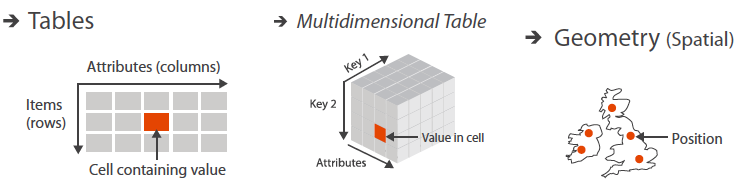
\includegraphics{figures/intro/munzner_datatypes}
    \label{fig:munzner_datatypes}
    \caption{Keys are unique lookup values used to find individual observations in the dataset. Keys are positional references, and can be coordinates on a map or unique values such as a primary key in a database or a (time, latitude, longitude) index in a data cube. Image modified from a diagram from Munzner's website\cite{munznerChDataAbstraction}}
\end{figure}

\cite{munznerWhatDataAbstraction2014}

\printbibliography
\end{document}